% Modified and remixed by Robert Hildebrand
% Source: https://math.libretexts.org/Bookshelves/Applied_Mathematics/Applied_Finite_Mathematics_(Sekhon_and_Bloom)
% License: CC BY 4.0 (Creative Commons Attribution 4.0 International)
% Authors: Rupinder Sekhon and Roberta Bloom

\chapter{Linear Equations}

\noindent\textit{This chapter is adapted from \emph{Applied Finite Mathematics} by Rupinder Sekhon and Roberta Bloom, available at
\url{https://math.libretexts.org/Bookshelves/Applied_Mathematics/Applied_Finite_Mathematics_(Sekhon_and_Bloom)},
licensed under \href{https://creativecommons.org/licenses/by/4.0/}{CC~BY~4.0}.
Content has been modified and remixed for this book.}

\medskip

\begin{outcome}
\begin{itemize}
\item Graph linear equations.
\item Find the slope of a line.
\item Determine equations of lines.
\item Solve linear systems.
\item Apply linear equations to real-world problems.
\end{itemize}
\end{outcome}

\section*{Chapter Overview}
In this chapter\footnote{This section was modified and remixed from 
Applied Finite Mathematics (Sekhon and Bloom)/Section 1.1: Graphing a linear equation which was shared under a CC BY 4.0 license at 
\url{https://math.libretexts.org/Bookshelves/Applied_Mathematics/Applied_Finite_Mathematics_(Sekhon_and_Bloom)/01\%3A_Linear_Equations/1.01\%3A_Graphing_a_Linear_Equation}
}, 
we focus on linear equations, their graphical representations, finding slopes, determining line equations from given information, and solving systems of linear equations. We also examine applications of these concepts in real-world scenarios, such as cost modeling, demand-supply equilibrium, and break-even analysis.

\section{Graphing a Linear Equation}
\begin{outcome}
\begin{itemize}
\item Graph a line from its equation.
\item Graph a line given its equation in parametric form.
\item Graph and find equations of vertical and horizontal lines.
\end{itemize}
\end{outcome}

Equations whose graphs are straight lines are called \emph{linear equations}. Examples include:
\[
2x - 3y = 6,\quad 3x = 4y - 7,\quad y = 2x - 5,\quad 2y = 3,\quad x - 2 = 0.
\]

A line is determined by two points. To graph a linear equation, we often choose values for one variable and solve for the other.

\begin{example}{Graphing a Line}\label{exa:line-graph1}
Graph the line: \(y = 3x + 2\).

\textbf{Solution:} Choose convenient $x$-values:
\[
x = -1 \implies y = 3(-1) + 2 = -1 \implies (-1,-1)
\]
\[
x = 0 \implies y = 3(0) + 2 = 2 \implies (0,2)
\]
\[
x = 1 \implies y = 3(1) + 2 = 5 \implies (1,5)
\]

Plot these points and draw the line.
\begin{center}
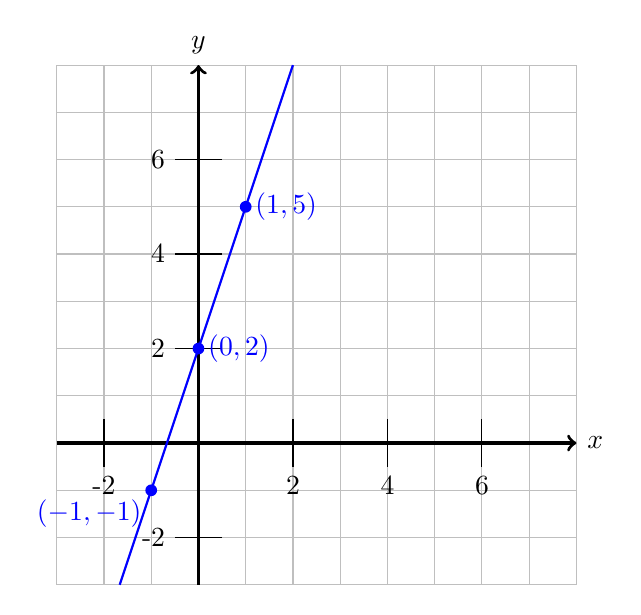
\begin{tikzpicture}[scale = 0.6]
    % Grid and axes
    \draw[gray!50, thin, step=1] (-3,-3) grid (8,8);
    \draw[very thick,->] (-3,0) -- (8,0) node[right] {$x$};
    \draw[very thick,->] (0,-3) -- (0,8) node[above] {$y$};

    % Axis labels
    \foreach \x in {-2,2,4,6} \draw (\x,0.5) -- (\x,-0.5) node[below] {\x};
    \foreach \y in {-2,2,4,6}  \draw (0.5,\y) -- (-0.5,\y) node[left] {\y};

    % Vertices
    \node[blue] at (-1,-1) [circle,fill,inner sep=1.5pt]{};
    \node[blue] at (0,2) [circle,fill,inner sep=1.5pt]{};
    \node[blue] at (1,5) [circle,fill,inner sep=1.5pt]{};
    

    % Labels for vertices
    \node[blue,anchor=north east] at (-1,-1) {$(-1,-1)$};
    \node[blue,anchor=west] at (0,2) {$(0,2)$};
    \node[blue,anchor=west] at (1,5) {$(1,5)$};
    
    \draw[blue, thick] (2,8) -- (-1.6667, -3);
\end{tikzpicture}
\end{center}
\end{example}

\begin{example}{Graphing Another Line}\label{exa:line-graph2}
Graph the line: \(2x + y = 4\).

\textbf{Solution:} Choose points:
\[
x = -1 \implies 2(-1) + y =4 \implies y =6 \implies (-1,6)
\]
\[
x = 0 \implies y =4 \implies (0,4)
\]
\[
y = 2 \implies 2x+2=4 \implies x=1 \implies (1,2)
\]

Plotting these points gives:
\begin{center}
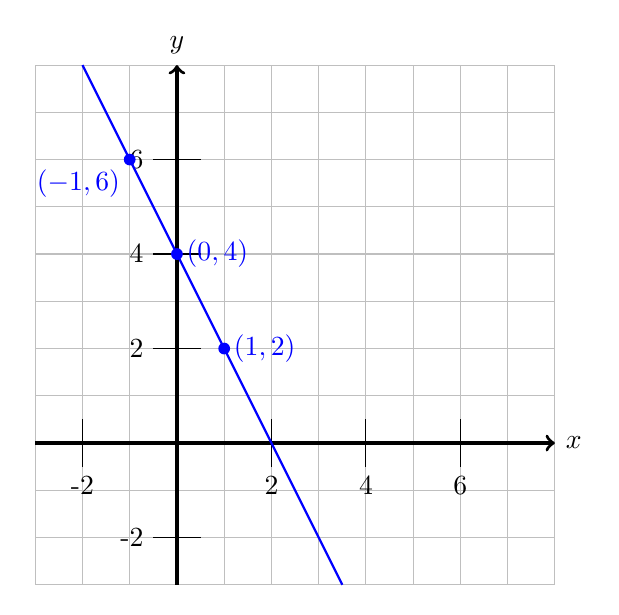
\begin{tikzpicture}[scale = 0.6]
    % Grid and axes
    \draw[gray!50, thin, step=1] (-3,-3) grid (8,8);
    \draw[very thick,->] (-3,0) -- (8,0) node[right] {$x$};
    \draw[very thick,->] (0,-3) -- (0,8) node[above] {$y$};

    % Axis labels
    \foreach \x in {-2,2,4,6} \draw (\x,0.5) -- (\x,-0.5) node[below] {\x};
    \foreach \y in {-2,2,4,6}  \draw (0.5,\y) -- (-0.5,\y) node[left] {\y};

    % Vertices
    \node[blue] at (-1,6) [circle,fill,inner sep=1.5pt]{};
    \node[blue] at (0,4) [circle,fill,inner sep=1.5pt]{};
    \node[blue] at (1,2) [circle,fill,inner sep=1.5pt]{};
    

    % Labels for vertices
    \node[blue,anchor=north east] at (-1,6) {$(-1,6)$};
    \node[blue,anchor=west] at (0,4) {$(0,4)$};
    \node[blue,anchor=west] at (1,2) {$(1,2)$};
    
    \draw[blue, thick] (-2,8) -- (3.5, -3);
\end{tikzpicture}
\end{center}
\end{example}

\subsection*{Intercepts}
The $x$-intercept occurs where $y=0$, and the $y$-intercept occurs where $x=0$.

\begin{example}{Finding Intercepts}\label{exa:intercepts}
Find the intercepts of the line \(2x - 3y = 6\) and graph it.

\textbf{Solution:} For the $x$-intercept, set $y=0$:
\[
2x -3(0)=6 \implies x=3 \implies (3,0).
\]

For the $y$-intercept, set $x=0$:
\[
2(0)-3y=6 \implies y=-2 \implies(0,-2).
\]

Plot these intercepts and draw the line.
\begin{center}
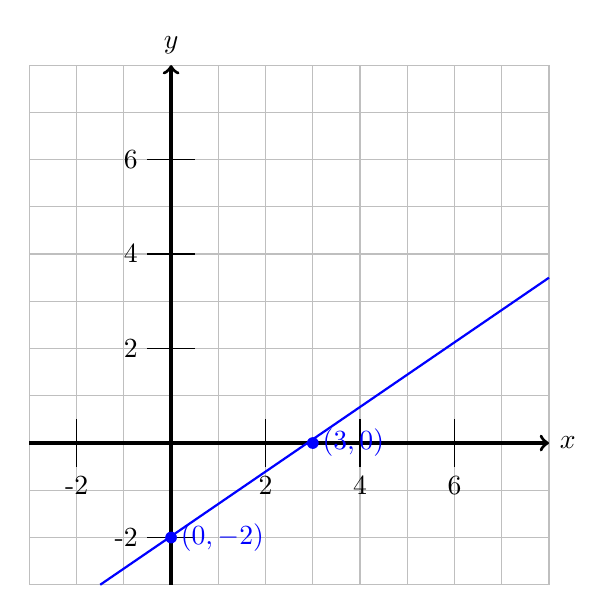
\begin{tikzpicture}[scale = 0.6]
    % Grid and axes
    \draw[gray!50, thin, step=1] (-3,-3) grid (8,8);
    \draw[very thick,->] (-3,0) -- (8,0) node[right] {$x$};
    \draw[very thick,->] (0,-3) -- (0,8) node[above] {$y$};

    % Axis labels
    \foreach \x in {-2,2,4,6} \draw (\x,0.5) -- (\x,-0.5) node[below] {\x};
    \foreach \y in {-2,2,4,6}  \draw (0.5,\y) -- (-0.5,\y) node[left] {\y};

    % Vertices
    \node[blue] at (0,-2) [circle,fill,inner sep=1.5pt]{};
    \node[blue] at (3,0) [circle,fill,inner sep=1.5pt]{};
    

    % Labels for vertices
    \node[blue,anchor=west] at (0,-2) {$(0,-2)$};
    \node[blue,anchor=west] at (3,0) {$(3,0)$};
    
    \draw[blue, thick] (-1.5,-3) -- (8, 3.5);
\end{tikzpicture}
\end{center}
\end{example}

\subsection*{Parametric Form}
Lines can also be given in parametric form, e.g. \(x=3+2t,\; y=1+t\).

\begin{example}{Parametric Equations}\label{exa:parametric-line}
Graph the line \(x=3+2t, y=1+t.\)

\textbf{Solution:} Let $t=0,1,2$:
\[
t=0 \implies (x,y)=(3,1), \quad t=1 \implies (5,2), \quad t=2 \implies (7,3).
\]

Plot these points and draw the line.
\begin{center}
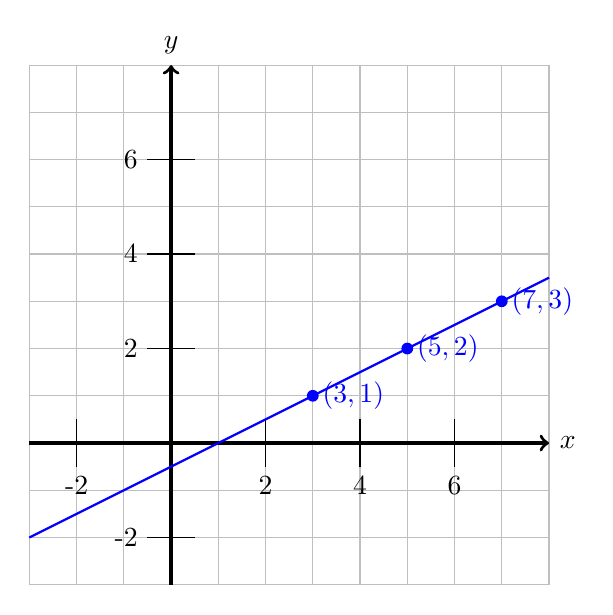
\begin{tikzpicture}[scale = 0.6]
    % Grid and axes
    \draw[gray!50, thin, step=1] (-3,-3) grid (8,8);
    \draw[very thick,->] (-3,0) -- (8,0) node[right] {$x$};
    \draw[very thick,->] (0,-3) -- (0,8) node[above] {$y$};

    % Axis labels
    \foreach \x in {-2,2,4,6} \draw (\x,0.5) -- (\x,-0.5) node[below] {\x};
    \foreach \y in {-2,2,4,6}  \draw (0.5,\y) -- (-0.5,\y) node[left] {\y};

    % Vertices
    \node[blue] at (3,1) [circle,fill,inner sep=1.5pt]{};
    \node[blue] at (5,2) [circle,fill,inner sep=1.5pt]{};
        \node[blue] at (7,3) [circle,fill,inner sep=1.5pt]{};

    % Labels for vertices
        \node[blue,anchor=west] at (3,1) {$(3,1)$};
    \node[blue,anchor=west] at (5,2) {$(5,2)$};
    \node[blue,anchor=west] at (7,3) {$(7,3)$};
    
    \draw[blue, thick] (-3,-2) -- (8, 3.5);
\end{tikzpicture}
\end{center}
\end{example}

\subsection*{Horizontal and Vertical Lines}
\[
x = a \text{ is a vertical line passing through }(a,0),\quad y = b \text{ is a horizontal line passing through }(0,b).
\]

\begin{example}{Horizontal and Vertical Lines}\label{exa:horiz-vert}
Graph \(x=-2\) and \(y=3\).

\textbf{Solution:} The line \(x=-2\) is vertical through \((-2,0)\).
The line \(y=3\) is horizontal through \((0,3)\).
\begin{center}
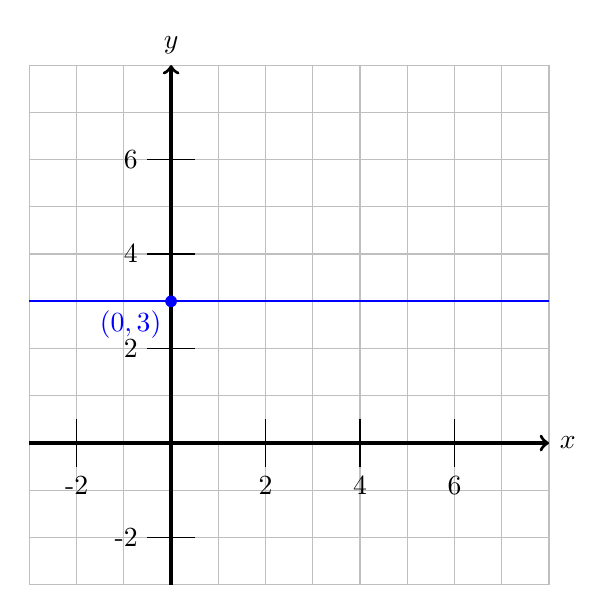
\begin{tikzpicture}[scale = 0.6]
    % Grid and axes
    \draw[gray!50, thin, step=1] (-3,-3) grid (8,8);
    \draw[very thick,->] (-3,0) -- (8,0) node[right] {$x$};
    \draw[very thick,->] (0,-3) -- (0,8) node[above] {$y$};

    % Axis labels
    \foreach \x in {-2,2,4,6} \draw (\x,0.5) -- (\x,-0.5) node[below] {\x};
    \foreach \y in {-2,2,4,6}  \draw (0.5,\y) -- (-0.5,\y) node[left] {\y};

    % Vertices
    \node[blue] at (0,3) [circle,fill,inner sep=1.5pt]{};
    
    % Labels for vertices
    \node[blue,anchor=north east] at (0,3) {$(0,3)$};
    
    \draw[blue, thick] (-3,3) -- (8, 3);
\end{tikzpicture}
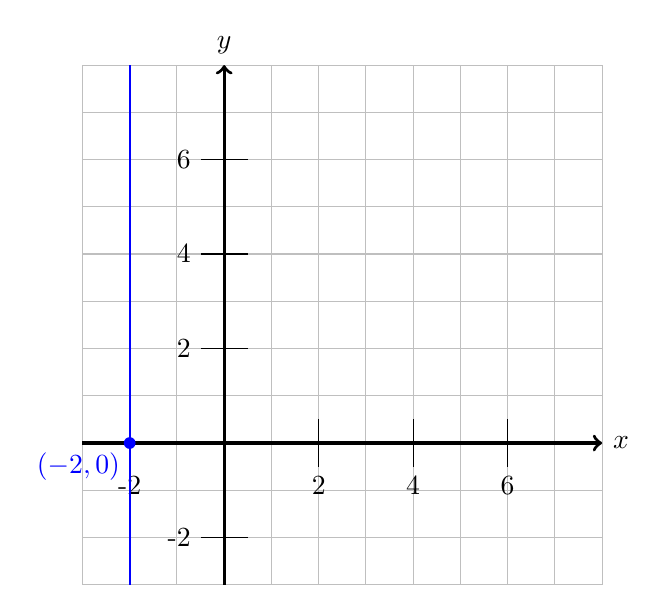
\begin{tikzpicture}[scale = 0.6]
    % Grid and axes
    \draw[gray!50, thin, step=1] (-3,-3) grid (8,8);
    \draw[very thick,->] (-3,0) -- (8,0) node[right] {$x$};
    \draw[very thick,->] (0,-3) -- (0,8) node[above] {$y$};

    % Axis labels
    \foreach \x in {-2,2,4,6} \draw (\x,0.5) -- (\x,-0.5) node[below] {\x};
    \foreach \y in {-2,2,4,6}  \draw (0.5,\y) -- (-0.5,\y) node[left] {\y};

    % Vertices
    \node[blue] at (-2,0) [circle,fill,inner sep=1.5pt]{};
    
    % Labels for vertices
    \node[blue,anchor=north east] at (-2,0) {$(-2,0)$};
    
    \draw[blue, thick] (-2,-3) -- (-2, 8);
\end{tikzpicture}
\end{center}
\end{example}

\section{Slope of a Line}
\begin{outcome}
\begin{itemize}
\item Find the slope of a line given two points.
\item Graph a line if a point and slope are given.
\end{itemize}
\end{outcome}

The slope \(m\) of a line passing through \((x_1,y_1)\) and \((x_2,y_2)\) is:
\[
m = \frac{y_2 - y_1}{x_2 - x_1}.
\]

\begin{example}{Finding Slope}\label{exa:slope1}
Find the slope of the line through \((-2,3)\) and \((4,-1)\).

\textbf{Solution:}
\[
m=\frac{-1-3}{4-(-2)}=\frac{-4}{6}=-\frac{2}{3}.
\]

\begin{center}
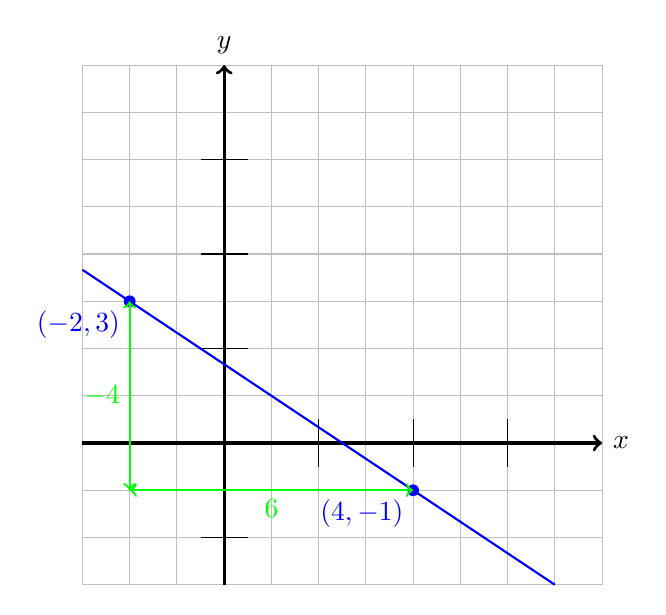
\begin{tikzpicture}[scale = 0.6]
    % Grid and axes
    \draw[gray!50, thin, step=1] (-3,-3) grid (8,8);
    \draw[very thick,->] (-3,0) -- (8,0) node[right] {$x$};
    \draw[very thick,->] (0,-3) -- (0,8) node[above] {$y$};

    % Axis labels
    \foreach \x in {-2,2,4,6} \draw (\x,0.5) -- (\x,-0.5) ;%node[below] {\x};
    \foreach \y in {-2,2,4,6}  \draw (0.5,\y) -- (-0.5,\y); %node[left] {\y};

    % Vertices
    \node[blue] at (-2,3) [circle,fill,inner sep=1.5pt]{};
    \node[blue] at (4,-1) [circle,fill,inner sep=1.5pt]{};
    

    % Labels for vertices
    \node[blue,anchor=north east] at (-2,3) {$(-2,3)$};
    \node[blue,anchor=north east] at (4,-1) {$(4,-1)$};
    
    \draw[blue, thick] (-3,3.6667) -- (7, -3);
    \draw[<->, green, thick] (-2,3) -- (-2,-1);
        \draw[<->, green, thick] (-2,-1) -- (4, -1);  
        
          \node[green,anchor= east] at (-2,1) {$-4$};
    \node[green,anchor=north ] at (1,-1) {$6$};
\end{tikzpicture}
\end{center}
\end{example}

Vertical lines have undefined slope; horizontal lines have slope 0.

\begin{example}{Vertical and Horizontal Slopes}\label{exa:vertical-horizontal-slope}
a) For points \((2,3)\) and \((2,-1)\):
\[
m=\frac{-1-3}{2-2}=\frac{-4}{0} \text{ (undefined), vertical line.}
\]

b) For points \((-1,-4)\) and \((3,-4)\):
\[
m=\frac{-4-(-4)}{3-(-1)}=\frac{0}{4}=0 \text{ (horizontal line).}
\]
\end{example}

\begin{example}{Graphing a Line from a Point and Slope}\label{exa:point-slope-graph}
Graph the line passing through \((1,2)\) with slope \(-\frac{3}{4}\).

\textbf{Solution:} Starting from \((1,2)\), a slope of \(-\frac{3}{4}\) means down 3, right 4 to get another point \((5,-1)\). Plot and draw the line.
\begin{center}
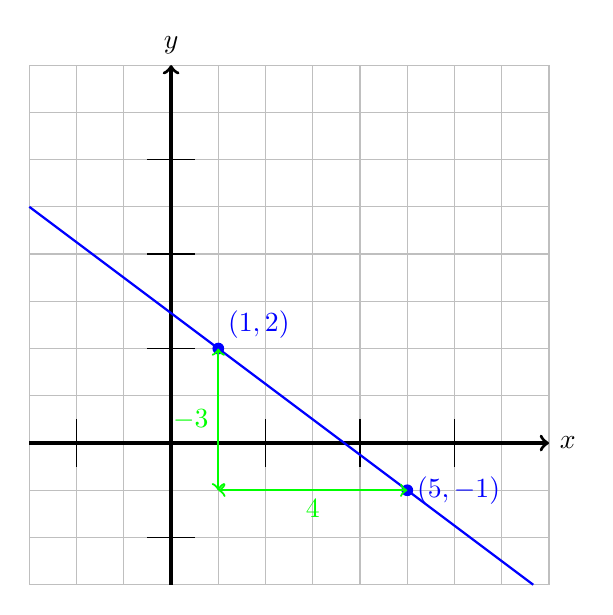
\begin{tikzpicture}[scale = 0.6]
    % Grid and axes
    \draw[gray!50, thin, step=1] (-3,-3) grid (8,8);
    \draw[very thick,->] (-3,0) -- (8,0) node[right] {$x$};
    \draw[very thick,->] (0,-3) -- (0,8) node[above] {$y$};

    % Axis labels
    \foreach \x in {-2,2,4,6} \draw (\x,0.5) -- (\x,-0.5);
    \foreach \y in {-2,2,4,6} \draw (0.5,\y) -- (-0.5,\y);

    % Vertices
    \node[blue] at (1,2) [circle,fill,inner sep=1.5pt]{};
    \node[blue] at (5,-1) [circle,fill,inner sep=1.5pt]{};

    % Labels for vertices
    \node[blue,anchor=south west] at (1,2) {$(1,2)$};
    \node[blue,anchor= west] at (5,-1) {$(5,-1)$};

    % Line through the points
    \draw[blue, thick] (-3,5) -- (7.6666,-3);

    % Slope indications
    \draw[<->, green, thick] (1,2) -- (1,-1);
    \draw[<->, green, thick] (1,-1) -- (5,-1);

    % Slope labels
    \node[green,anchor=east] at (1,0.5) {$-3$};
    \node[green,anchor=north] at (3,-1) {$4$};
\end{tikzpicture}
\end{center}
\end{example}

If a line is written as \(y=mx+b\), the coefficient \(m\) is the slope and \(b\) is the $y$-intercept.

\section{Determining the Equation of a Line}
\begin{outcome}
\begin{itemize}
\item Find an equation of a line given a point and slope.
\item Find an equation of a line given two points.
\end{itemize}
\end{outcome}

\subsection*{Forms of a Line}
\[
\text{Slope-Intercept: }y=mx+b,\quad \text{Point-Slope: }y-y_1=m(x-x_1),\quad \text{Standard: }Ax+By=C.
\]

\begin{example}{Equation Given Slope and Intercept}\label{exa:eq-slope-int}
Find the equation of a line with slope \(m=5\) and $y$-intercept \(b=3\).

\textbf{Solution:} \(y=5x+3.\)
\end{example}

\begin{example}{Equation Given a Point and Slope}\label{exa:eq-point-slope}
Find the equation of the line passing through \((2,7)\) with slope \(3\).

\textbf{Solution:}
\[
y=3x+b,\; 7=3(2)+b,\; b=1 \implies y=3x+1.
\]
\end{example}

\begin{example}{Equation Given Two Points}\label{exa:eq-two-points}
Find the equation of the line passing through \((-1,2)\) and \((1,8)\).

\textbf{Solution:}
\[
m=\frac{8-2}{1-(-1)}=\frac{6}{2}=3,\; y=3x+b.
\]
Use one point:
\[
2=3(-1)+b \implies b=5,\; \text{so } y=3x+5.
\]
\end{example}

\begin{example}{Using Intercepts}\label{exa:eq-from-intercepts}
Find the equation of the line with $x$-intercept 3 and $y$-intercept 4.

\textbf{Solution:} Intercepts give points $(3,0)$ and $(0,4)$:
\[
m=\frac{4-0}{0-3}=-\frac{4}{3},\;y=-\frac{4}{3}x+4.
\]
\end{example}

\section{Applications of Linear Equations}
\begin{outcome}
\begin{itemize}
\item Use linear functions to model real-world applications.
\end{itemize}
\end{outcome}

Linear equations commonly model cost, revenue, and population changes.

\begin{example}{Cost Function}\label{exa:cost-function}
A taxi charges \$0.50 per mile plus a \$5 flat fee.

\textbf{Solution:} Let $x=$ miles, $y=$ cost:
\[
y=0.50x+5.
\]
At $x=20$: $y=0.50(20)+5=15.$
\end{example}

\begin{example}{Cost from Two Points}\label{exa:cost-two-points}
It costs \$750 to make 25 items and \$1000 to make 50 items. Assume linearity.

\textbf{Solution:} Points $(25,750)$ and $(50,1000)$:
\[
m=\frac{1000-750}{50-25}=10,\;y=10x+b.
\]
Using $(25,750)$:
\[
750=10(25)+b \implies b=500,\;y=10x+500.
\]
Cost of 100 items: $y=10(100)+500=1500.$
\end{example}

\begin{example}{Temperature Conversion}\label{exa:temp-conversion}
Freezing point of water: $(C,F)=(0,32)$; boiling point: $(100,212)$.

\textbf{Solution:}
\[
m=\frac{212-32}{100-0}=\frac{180}{100}=1.8,\;F=1.8C+32.
\]
For $C=30$: $F=1.8(30)+32=86.$
\end{example}

\section{More Applications: Systems of Linear Equations}
\begin{outcome}
\begin{itemize}
\item Solve linear systems in two variables.
\item Find equilibrium points (supply = demand).
\item Find break-even points (cost = revenue).
\end{itemize}
\end{outcome}

\subsection*{Solving Systems of Equations}
The intersection of two lines can be found by setting their equations equal or by using the elimination method.

\begin{example}{Solving a System}\label{exa:system-solve}
Solve:
\[
2x+y=7,\quad 3x-y=3.
\]

\textbf{Solution:} Add them:
\[
2x+y=7,\;3x-y=3 \implies 5x=10 \implies x=2.
\]
Substitute $x=2$ into $2x+y=7 \implies 4+y=7 \implies y=3.$

Solution: $(2,3)$.
\end{example}

\subsection*{Supply, Demand, and Equilibrium}
The \emph{equilibrium price} occurs where supply equals demand.

\begin{example}{Equilibrium Point}\label{exa:equilibrium}
Supply: $y=3.5x-14$, Demand: $y=-2.5x+34$.

\textbf{Solution:} Set equal:
\[
3.5x-14=-2.5x+34 \implies 6x=48 \implies x=8.
\]
At $x=8$: $y=3.5(8)-14=14$ or $y=-2.5(8)+34=14$.

Equilibrium: Price = \$8, Quantity = 14 items.

\begin{center}
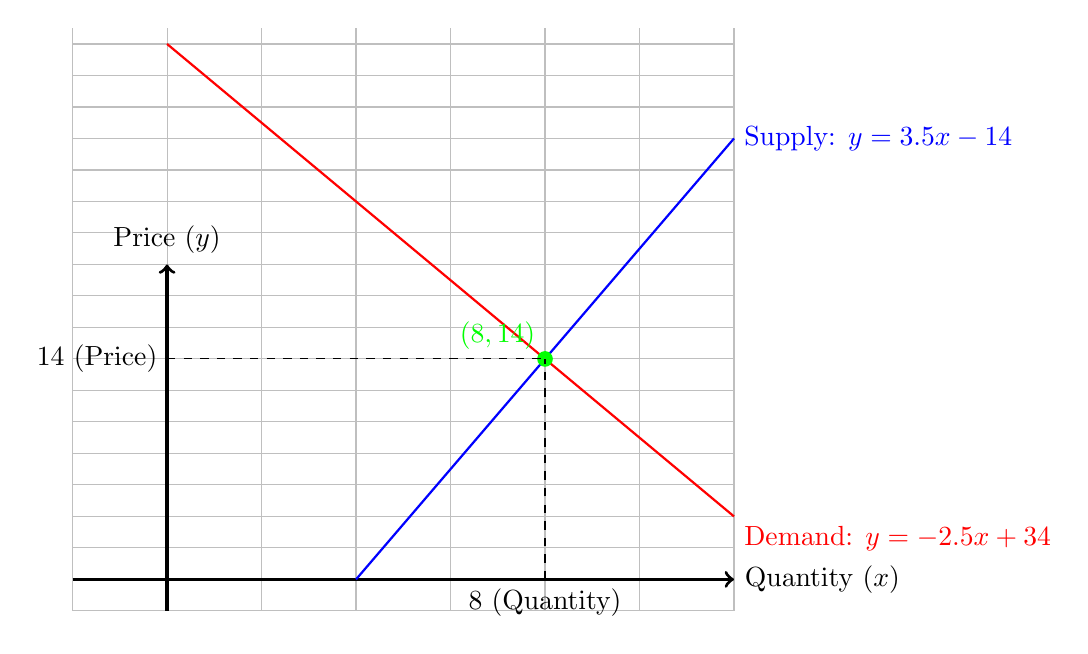
\begin{tikzpicture}[xscale=0.6, yscale=0.2]
    % Grid and axes
    \draw[gray!50, thin, step=2] (-2,-2) grid (12,35);
    \draw[very thick,->] (-2,0) -- (12,0) node[right] {Quantity ($x$)};
    \draw[very thick,->] (0,-2) -- (0,20) node[above] {Price ($y$)};

    % Supply line: y = 3.5x - 14
    \draw[blue, thick] (4,0) -- (12,28) node[anchor=west] {Supply: $y=3.5x-14$};

    % Demand line: y = -2.5x + 34
    \draw[red, thick] (0,34) -- (12,4) node[anchor=north west] {Demand: $y=-2.5x+34$};

    % Intersection point
    \node[green] at (8,14) [circle,fill,inner sep=2pt]{};
    \node[green,anchor=south east] at (8,14) {$(8,14)$};

    % Vertical and horizontal dashed lines to axes
    \draw[dashed] (8,0) -- (8,14);
    \draw[dashed] (0,14) -- (8,14);

    % Labels for equilibrium
    \node[anchor=north] at (8,0) {8 (Quantity)};
    \node[anchor=east] at (0,14) {14 (Price)};
\end{tikzpicture}
\end{center}
\end{example}

\subsection*{Break-Even Point}
For cost $C$ and revenue $R$, the break-even point is where $C=R$.

\begin{example}{Break-Even Analysis}\label{exa:break-even}
$R=5x$, $C=3x+12$.

\textbf{Solution:}
\[
5x=3x+12 \implies 2x=12 \implies x=6.
\]
At $x=6$, $R=C=30$.

Break-even at $(6,30)$.
\begin{center}
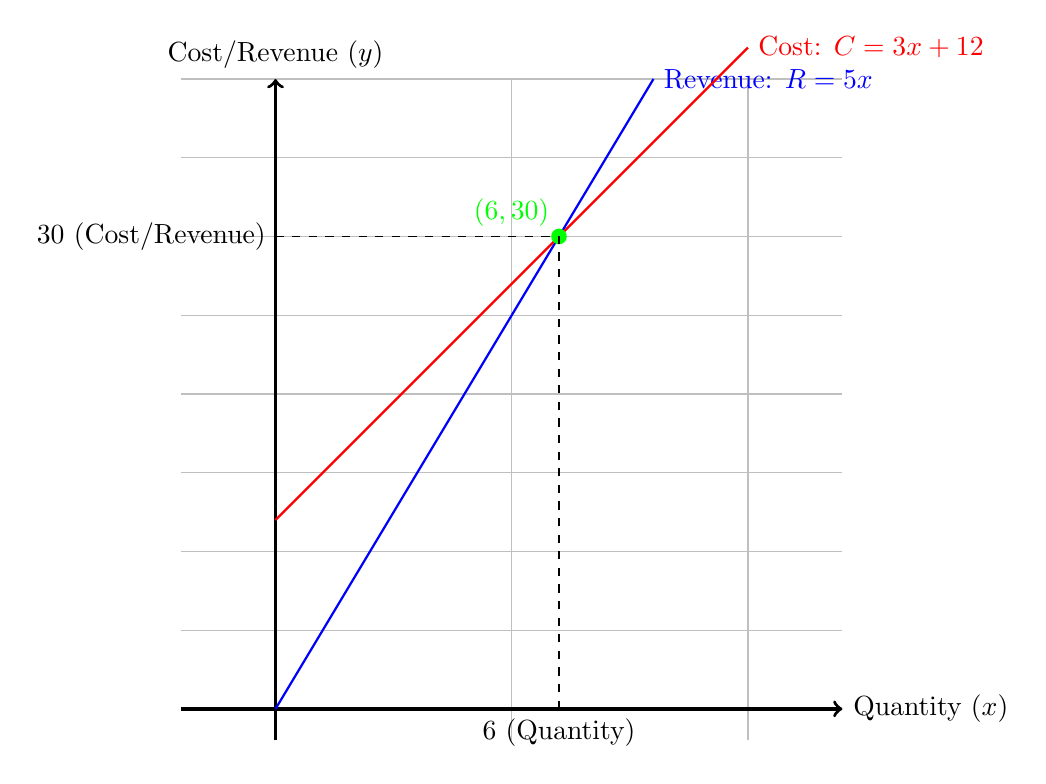
\begin{tikzpicture}[xscale=0.6, yscale=0.2]

    % Grid and axes
    \draw[gray!50, thin, step=5] (-2,-2) grid (12,40);
    \draw[very thick,->] (-2,0) -- (12,0) node[right] {Quantity ($x$)};
    \draw[very thick,->] (0,-2) -- (0,40) node[above] {Cost/Revenue ($y$)};

    % Revenue line: R = 5x
    \draw[blue, thick] (0,0) -- (8,40) node[anchor=west] {Revenue: $R=5x$};

    % Cost line: C = 3x + 12
    \draw[red, thick] (0,12) -- (10,42) node[anchor=west] {Cost: $C=3x+12$};

    % Break-even point
    \node[green] at (6,30) [circle,fill,inner sep=2pt]{};
    \node[green,anchor=south east] at (6,30) {$(6,30)$};

    % Vertical and horizontal dashed lines to axes
    \draw[dashed] (6,0) -- (6,30);
    \draw[dashed] (0,30) -- (6,30);

    % Labels for break-even
    \node[anchor=north] at (6,0) {6 (Quantity)};
    \node[anchor=east] at (0,30) {30 (Cost/Revenue)};
\end{tikzpicture}
\end{center}
\end{example}

\section*{Chapter Review}
This chapter introduced the fundamental concepts of linear equations, their graphs, slopes, forms of equations, and their real-world applications. You can now model scenarios involving costs, pricing, and market equilibrium using linear models and solve these models for key insights.
